\section{Part 3 -- Acceleo}

\subsection{Definition of the Acceleo Program}

The Acceleo program that we developed takes as input an XMI file containing a representation of the model in a suitable way for Acceleo, initially generated by OSATE as an AAXL2 file representing an instance of a system.
In order to use this data as input to Acceleo, we used pre-built EMF meta-models for AADL, found in the \texttt{aadl.ecore} and \texttt{instance.ecore} model.

After integrating the XMI file in Acceleo, we are able to generate code applying an M2T transformation. At this point we can generate a text/HTML file containing a possible representation of our model.

\subsection{Example of output}

\begin{figure}[h]
\caption{Product of the Acceleo code generation}
\label{fig:html}
\centering
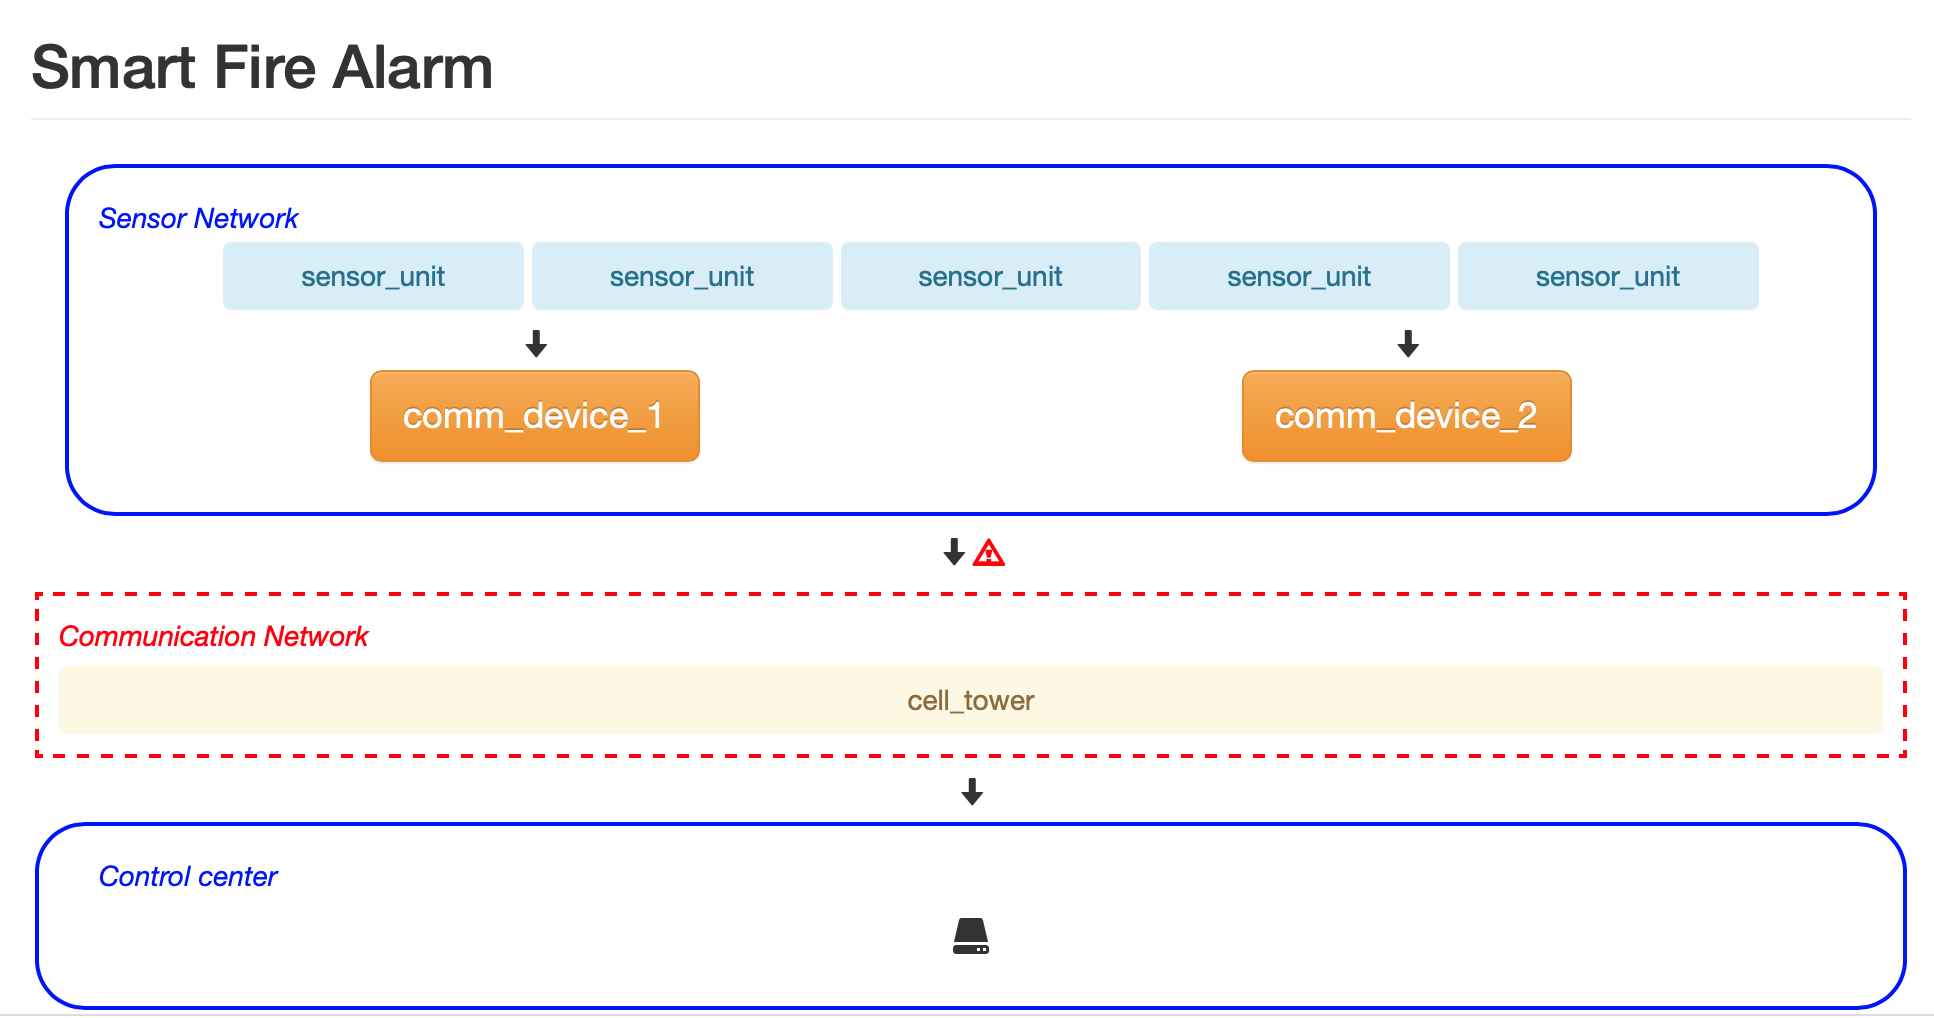
\includegraphics[width=0.45\textwidth]{html}
\end{figure}

Our Acceleo program outputs an HTML page containing a dynamic diagram which represents the basic flow between the components of the model. 
The components are grouped in three blocks: Sensor Network, Communication Network and Control Center.
The sensor units defined in the instance are located inside the Sensor Network, and they send data to the communication devices. 
The Sensor Network can send data and/or an alarm signal to the Communication Network block, which will forward it to the Control Center. 
\autoref{fig:html} is a screen capture of the product of the code generation process.

This is an example of the various types of representations that can be made.
The view was made inserting the various components into HTML code, exploiting Bootstrap.
Names of components are extracted from from the XMI file by iterating through the various elements contained within.
In fact, in the XMI file it is possible to find the tags for every component, flow and connection in the model.